
\documentclass[11pt]{article}

% ------------------------------------------------------------
% Standard LaTeX packages
% ------------------------------------------------------------
\usepackage[margin=1in]{geometry}
\usepackage{lmodern}
\usepackage{amsmath,amssymb,mathtools}
\usepackage{amsthm}
\usepackage[american]{babel}
\usepackage{enumitem}
\usepackage{booktabs}
\usepackage{array}
\usepackage{url}
\usepackage{tikz}
\usetikzlibrary{positioning,arrows.meta,shapes.geometric,calc,fit,backgrounds}
\usepackage[colorlinks=true,linkcolor=blue,citecolor=blue,urlcolor=blue]{hyperref}

% ---------- Theorem environments ----------
\theoremstyle{plain}
\newtheorem{theorem}{Theorem}[section]
\newtheorem{proposition}[theorem]{Proposition}
\newtheorem{lemma}[theorem]{Lemma}
\newtheorem{corollary}[theorem]{Corollary}

\theoremstyle{definition}
\newtheorem{definition}[theorem]{Definition}
\newtheorem{example}[theorem]{Example}
\newtheorem{observation}[theorem]{Observation}

\theoremstyle{remark}
\newtheorem{remark}[theorem]{Remark}

% ---------- Mathematical notation ----------
\newcommand{\N}{\mathbb{N}}
\newcommand{\Z}{\mathbb{Z}}
\newcommand{\Q}{\mathbb{Q}}
\newcommand{\R}{\mathbb{R}}
\newcommand{\C}{\mathbb{C}}
\newcommand{\F}{\mathbb{F}}
\newcommand{\Qbar}{\overline{\Q}}
\newcommand{\Qell}{\Q_\ell}
\newcommand{\Qp}{\Q_p}
\newcommand{\Fq}{\mathbb{F}_q}
\newcommand{\BISH}{\mathrm{BISH}}
\newcommand{\LPO}{\mathrm{LPO}}
\newcommand{\WLPO}{\mathrm{WLPO}}
\newcommand{\LLPO}{\mathrm{LLPO}}
\newcommand{\CRM}{\mathrm{CRM}}
\newcommand{\CLASS}{\mathrm{CLASS}}
\newcommand{\FT}{\mathrm{FT}}
\newcommand{\MP}{\mathrm{MP}}
\newcommand{\DC}{\mathrm{DC}}

% ---------- Title and author ----------
\title{Decidability, Visibility, and the Architecture\\
of Mathematical Truth:\\[4pt]
A Synthesis of the Constructive Reverse\\
Mathematics Program\\[6pt]
\large (Paper~54, Constructive Reverse Mathematics Series)}

\author{Paul Chun-Kit Lee \\
New York University \\
\texttt{dr.paul.c.lee@gmail.com}}

\date{February 2026}

\begin{document}
\maketitle

\begin{abstract}
This paper synthesizes the constructive reverse mathematics (CRM) program developed across Papers~1--53 of this series.  The program calibrates mathematical theorems against logical principles---$\BISH$, $\WLPO$, $\LPO$, $\MP$, $\FT$---revealing three structurally distinct obstructions to computation: \emph{logical} (omniscience principles, Papers~2--31), \emph{geometric} (visibility failures in the Lefschetz ring, Papers~52--53), and \emph{Diophantine} (irreducible Markov search, Papers~45--51).  The undecidability genealogy (Papers~29--42) advances the thesis that empirical physics requires exactly $\BISH + \LPO$: every physical undecidability result calibrated in the series---including the spectral gap---is $\LPO$-equivalent, traceable to Wang tiling.  Markov's Principle governs the residual cost of physical actualisation (Paper~43).  In arithmetic geometry, the Standard Conjectures function as decidability axioms (ensuring decidable equivalence relations on cycle spaces), the motive is a decidability certificate, and the dimension-4 boundary for abelian varieties is sharp---confirmed computationally ($\deg(w \cdot w) = 7 > 0$).  No new formal theorems are proved; this is an interpretive essay drawing on 53~papers, 12 with Lean~4 formalizations.  It does, however, propose novel interpretive frameworks---particularly the obstruction trichotomy and the de-omniscientizing descent pattern---that organize the prior results in ways not explicit in the individual papers.
\end{abstract}

\tableofcontents


%% ===================================================================
\section{Introduction}
\label{sec:intro}
%% ===================================================================

\subsection{The program}

Over the course of 53~papers, the constructive reverse mathematics program has asked a single question of each theorem it encounters: \emph{what logical resources does this theorem actually require?}

The question is not idle.  Classical mathematics proves theorems from the law of excluded middle and the axiom of choice, treating all proofs as equal consumers of these resources.  Constructive reverse mathematics ($\CRM$) refines this: it identifies a hierarchy of principles---$\BISH$ (Bishop-style constructive mathematics, no omniscience), $\WLPO$ (Weak Limited Principle of Omniscience), $\LPO$ (Limited Principle of Omniscience), and full $\CLASS$ (classical logic)---and determines where each theorem \emph{naturally lives} in this hierarchy.

The result, accumulated across 53~papers, is a calibration atlas: a map of mathematical theorems plotted against their logical coordinates.  The atlas spans functional analysis (Papers~2, 7~\cite{Paper2,Paper7}), quantum mechanics (Paper~6~\cite{Paper6}), statistical physics (Paper~8~\cite{Paper8}), optimization theory (Paper~23~\cite{Paper23}), classical mechanics (Paper~28~\cite{Paper28}), and arithmetic geometry (Papers~45--53~\cite{Paper51,Paper52,Paper53}).

\subsection{The central discovery}

The program's most unexpected finding is that \emph{obstructions to computation are not uniform}.  Three structurally distinct types emerge:

\begin{description}[leftmargin=2em]
\item[Logical obstructions.] The theorem genuinely requires an omniscience principle.  The bidual gap for Banach spaces is equivalent to~$\WLPO$ (Paper~2); the thermodynamic limit of the 1D~Ising model is equivalent to~$\LPO$ (Paper~8).  These are irreducible: no cleverness removes the need for omniscience.

\item[Geometric obstructions.] The mathematical structure hides information from the decidability machinery.  The exotic Weil class on a CM abelian fourfold is algebraic, has positive self-intersection, and satisfies the Hodge--Riemann relations---it is computationally healthy---but lies outside the Lefschetz ring where the decidability oracle operates (Papers~52, 53).  The obstruction is \emph{visibility}, not pathology.

\item[Diophantine obstructions.] A search through an unbounded space is irreducible.  The Birch--Swinnerton-Dyer generator search requires Markov's Principle ($\MP$), which no amount of algebraic structure eliminates (Paper~51).  The motive kills~$\LPO$ but not~$\MP$.
\end{description}

\begin{figure}[ht]
\centering
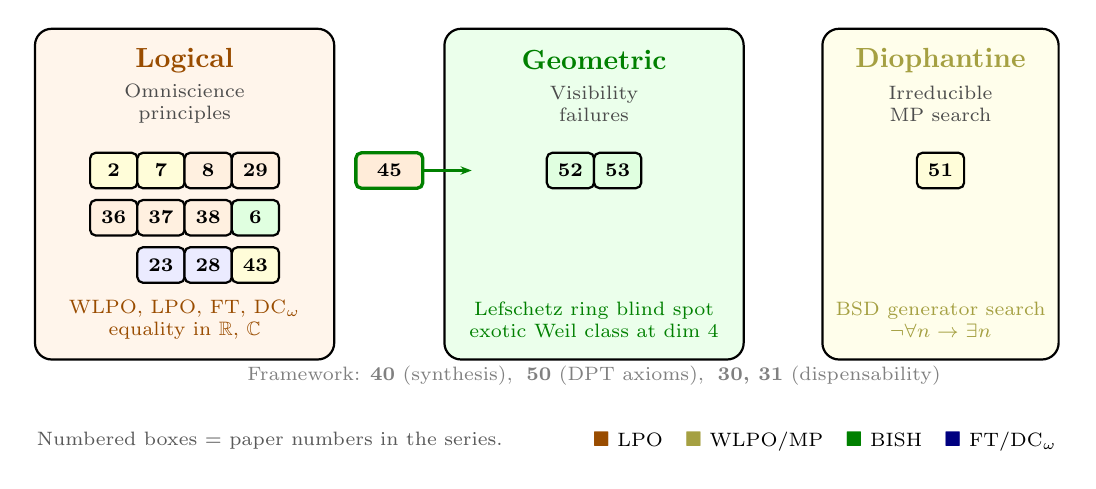
\begin{tikzpicture}[
  every node/.style={font=\small},
  region/.style={draw, thick, rounded corners=6pt, minimum height=4.2cm,
                 align=center},
  paperdot/.style={draw, fill=white, rounded corners=2pt, thick,
                   minimum width=0.6cm, minimum height=0.45cm,
                   font=\scriptsize\bfseries, inner sep=2pt},
  rlabel/.style={font=\normalsize\bfseries, align=center},
  desc/.style={font=\scriptsize, text=gray!60!black, align=center, text width=3.0cm}
]

  % --- Three regions ---
  \node[region, fill=orange!8, minimum width=3.8cm] (logical) at (0, 0) {};
  \node[region, fill=green!8,  minimum width=3.8cm] (geometric) at (5.2, 0) {};
  \node[region, fill=yellow!8, minimum width=3.0cm] (diophantine) at (9.6, 0) {};

  % --- Region titles ---
  \node[rlabel, text=orange!60!black] at (0, 1.7) {Logical};
  \node[rlabel, text=green!50!black]  at (5.2, 1.7) {Geometric};
  \node[rlabel, text=yellow!60!black] at (9.6, 1.7) {Diophantine};

  % --- Subtitles ---
  \node[desc] at (0, 1.15) {Omniscience\\principles};
  \node[desc] at (5.2, 1.15) {Visibility\\failures};
  \node[desc] at (9.6, 1.15) {Irreducible\\$\MP$ search};

  % --- Papers in Logical region ---
  \node[paperdot, fill=yellow!15] at (-0.9, 0.3)  {2};
  \node[paperdot, fill=yellow!15] at (-0.3, 0.3)  {7};
  \node[paperdot, fill=orange!12] at (0.3, 0.3)   {8};
  \node[paperdot, fill=orange!12] at (0.9, 0.3)   {29};
  \node[paperdot, fill=orange!12] at (-0.9, -0.3) {36};
  \node[paperdot, fill=orange!12] at (-0.3, -0.3) {37};
  \node[paperdot, fill=orange!12] at (0.3, -0.3)  {38};
  \node[paperdot, fill=green!12]  at (0.9, -0.3)  {6};
  \node[paperdot, fill=blue!8]    at (-0.3, -0.9) {23};
  \node[paperdot, fill=blue!8]    at (0.3, -0.9)  {28};
  \node[paperdot, fill=yellow!15] at (0.9, -0.9)  {43};

  % --- Papers in Geometric region ---
  \node[paperdot, fill=green!12] at (4.9, 0.3)  {52};
  \node[paperdot, fill=green!12] at (5.5, 0.3)  {53};

  % --- Papers in Diophantine region ---
  \node[paperdot, fill=yellow!15] at (9.6, 0.3) {51};

  % --- Transition zone: Paper 45 straddles Logical and Geometric ---
  \node[paperdot, fill=orange!15, draw=green!50!black, very thick,
        minimum width=0.85cm] (p45) at (2.6, 0.3) {45};
  \draw[-{Stealth[length=4pt]}, thick, green!50!black]
    (p45.east) -- +(0.6, 0);

  % --- Mechanism labels below regions ---
  \node[font=\scriptsize, text=orange!60!black, align=center] at (0, -1.6)
    {$\WLPO$, $\LPO$, $\FT$, $\DC_\omega$\\equality in $\R$, $\C$};
  \node[font=\scriptsize, text=green!50!black, align=center] at (5.2, -1.6)
    {Lefschetz ring blind spot\\exotic Weil class at dim~4};
  \node[font=\scriptsize, text=yellow!60!black, align=center] at (9.6, -1.6)
    {BSD generator search\\$\lnot\forall n \to \exists n$};

  % --- Framework papers annotation ---
  \node[font=\scriptsize, text=gray, align=center] at (5.2, -2.3)
    {Framework: \textbf{40}~(synthesis),\; \textbf{50}~(DPT axioms),\; \textbf{30, 31}~(dispensability)};

  % --- Legend (bottom-left) ---
  \node[anchor=north west, font=\scriptsize, text=gray!70!black, align=left] at (-2.0, -2.9)
    {Numbered boxes = paper numbers in the series.};

  % --- Color key (bottom-right) ---
  \node[anchor=north east, align=right, font=\scriptsize] at (11.2, -2.9) {%
    \textcolor{orange!60!black}{$\blacksquare$}~$\LPO$\quad
    \textcolor{yellow!60!black}{$\blacksquare$}~$\WLPO$/$\MP$\quad
    \textcolor{green!50!black}{$\blacksquare$}~$\BISH$\quad
    \textcolor{blue!50!black}{$\blacksquare$}~$\FT$/$\DC_\omega$};

\end{tikzpicture}
\caption{The obstruction trichotomy.  Numbered boxes identify papers
in the series; box colors indicate the CRM strength of each paper's
main result (see color key).
Logical obstructions (left) require
omniscience principles; geometric obstructions (center) arise from
visibility failures in the Lefschetz ring; Diophantine obstructions (right)
are irreducible Markov searches.  Paper~45 straddles the logical--geometric
boundary: its abstract formulation is~$\LPO$, but geometric origin reduces it
to~$\BISH$.}
\label{fig:trichotomy}
\end{figure}

This trichotomy was not anticipated at the start of the program.  Papers~2--28 found only logical obstructions; Papers~29--42 unified these into the $\BISH + \LPO$ characterization (\S\ref{sec:constitution}).  The geometric type emerged only when the program reached arithmetic geometry (Papers~45--53), where the interplay between logic and geometry produces a richer obstruction theory.

\subsection{Three audiences}

This synthesis addresses three communities simultaneously:

\begin{itemize}[nosep]
\item \textbf{Physicists} will find that the CRM calibration reveals genuine computational structure in physics.  The preparation uncertainty principle requires no omniscience; measurement uncertainty does.  Finite thermodynamic bounds are constructive; the infinite-volume limit is not.  These are not artifacts of formalism---they track the difference between what a finite machine can compute and what requires idealized infinite operations.

\item \textbf{Philosophers of mathematics} will find a landscape finer than the classical decidable/undecidable dichotomy.  There are at least four levels ($\BISH$, $\WLPO$, $\LPO$, $\CLASS$), plus independent axes ($\FT$, $\DC_\omega$).  The dimension-4 obstruction admits a Kantian reading.  The emergence of geometric (as opposed to logical) obstructions is philosophically novel.

\item \textbf{Arithmetic geometers} will find that Grothendieck's Standard Conjectures acquire a precise logical characterization: they are decidability axioms, ensuring that the equivalence relation on cycle spaces reduces from~$\LPO$ to~$\BISH$.  The motive is a decidability certificate.  Standard Conjecture~D is the condition making the equivalence relation on morphism spaces decidable (though effective computation of the full morphism spaces requires additional input such as explicit cycle bases).  The dimension-4 boundary for the DPT framework is sharp, confirmed computationally.
\end{itemize}

\subsection{Structure of this essay}

Section~\ref{sec:geography} presents the logical geography---the hierarchy and the calibration table.  Section~\ref{sec:constitution} describes the $\BISH + \LPO$ characterization and the undecidability genealogy (Papers~29--42).  Section~\ref{sec:descent} describes the de-omniscientizing descent pattern that unifies the five great conjectures (Papers~45--50).  Section~\ref{sec:wall} analyzes the dimension-4 wall.  Sections~\ref{sec:physics},~\ref{sec:philosophy}, and~\ref{sec:ag} draw out the implications for physics, philosophy, and arithmetic geometry respectively.  Section~\ref{sec:retrospect} reflects on the program as a whole.  Section~\ref{sec:conclusion} offers a brief conclusion.

\subsection{Epistemic status}

The calibrations presented in this series, and the interpretations offered in this synthesis, should be regarded as preliminary.  The CRM methodology---applying constructive reverse mathematics to theorems outside its traditional domain---is not standard practice in any of the three communities addressed here.  Professional logicians, arithmetic geometers, and mathematical physicists may reasonably disagree with our interpretations of which logical principles a given theorem ``requires,'' particularly when the formalization involves axiom-as-hypothesis patterns or when the obstruction classification (logical vs.\ geometric) relies on informal judgments about proof structure.

This essay represents how the author interprets the accumulated data from 53~calibrations.  It is offered as a contribution to an ongoing conversation, not as a definitive account.


%% ===================================================================
\section{The Logical Geography}
\label{sec:geography}
%% ===================================================================

\subsection{The hierarchy}

The logical principles relevant to this program form a \emph{partial order}---not a linear chain:
\[
\BISH \;\subset\; \BISH + \WLPO \;\subset\; \BISH + \LPO \;\subset\; \CLASS.
\]
Here~$\BISH$ is Bishop's constructive mathematics~\cite{BridgesRichman1987}: intuitionistic logic, countable choice, no omniscience.  $\WLPO$ asserts that every binary sequence is identically zero or has a nonzero term---but does not tell you \emph{which} term (existence without witness).  $\LPO$ strengthens this: every binary sequence either is identically zero or \emph{contains a~$1$ at a specific index} (existence with witness).  Classical logic ($\CLASS$) includes full excluded middle.

Critically, $\WLPO$ and $\MP$ are \emph{incomparable} over~$\BISH$: neither implies the other.  Together they recover $\LPO$:
\[
\BISH + \WLPO + \MP \;=\; \BISH + \LPO.
\]
The hierarchy therefore branches into a diamond (Figure~\ref{fig:diamond}).

\begin{figure}[ht]
\centering
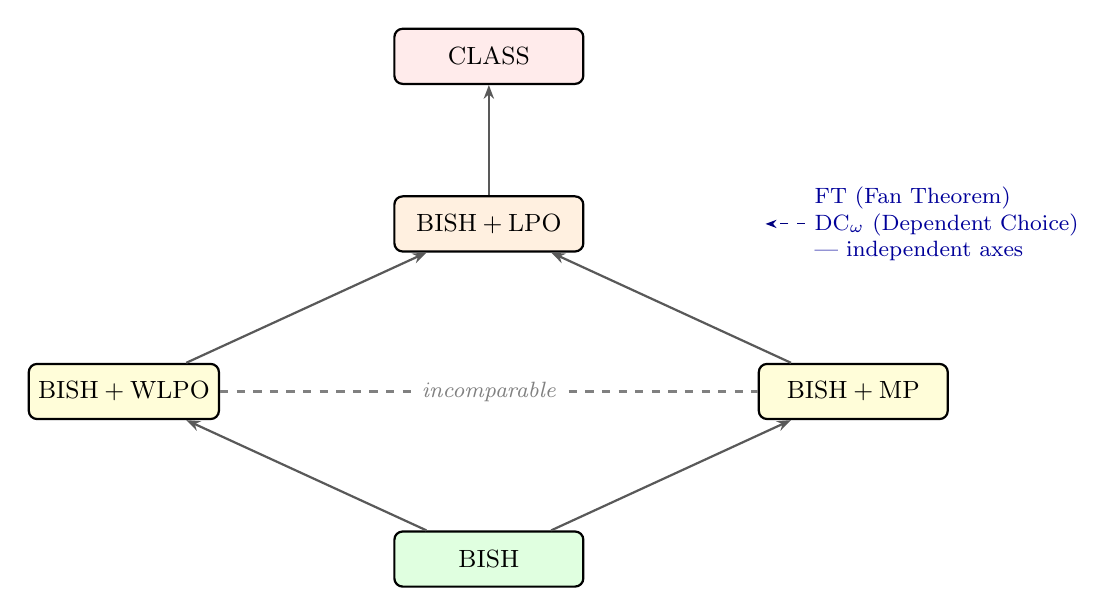
\begin{tikzpicture}[
  node distance=1.4cm and 2.2cm,
  every node/.style={font=\small},
  level/.style={draw, rounded corners=3pt, minimum width=2.4cm,
                minimum height=0.7cm, align=center, thick},
  impl/.style={-{Stealth[length=5pt]}, thick, gray!70!black}
]
  \node[level, fill=red!8]   (class) {$\CLASS$};
  \node[level, fill=orange!12, below=of class] (lpo)   {$\BISH + \LPO$};
  \node[level, fill=yellow!15, below left=of lpo]  (wlpo)  {$\BISH + \WLPO$};
  \node[level, fill=yellow!15, below right=of lpo] (mp)    {$\BISH + \MP$};
  \node[level, fill=green!12, below right=of wlpo] (bish)  {$\BISH$};

  \draw[impl] (bish) -- (wlpo);
  \draw[impl] (bish) -- (mp);
  \draw[impl] (wlpo) -- (lpo);
  \draw[impl] (mp)   -- (lpo);
  \draw[impl] (lpo)  -- (class);

  % incomparability annotation
  \draw[dashed, gray, thick] (wlpo) -- node[midway, fill=white, font=\footnotesize\itshape] {incomparable} (mp);

  % side annotations for independent axes
  \node[right=2.8cm of lpo, font=\footnotesize, text=blue!60!black, align=left]
    (ft) {$\FT$ (Fan Theorem)\\$\DC_\omega$ (Dependent Choice)\\--- independent axes};
  \draw[-{Stealth[length=4pt]}, dashed, blue!50!black, thin]
    (ft.west) -- +(-0.5,0);
\end{tikzpicture}
\caption{The CRM diamond.  Arrows denote strict implication over~$\BISH$.
$\WLPO$ and~$\MP$ are incomparable; their join is~$\LPO$.
The Fan Theorem and Dependent Choice are independent of the main spine.}
\label{fig:diamond}
\end{figure}

\noindent
The CRM program tracks which of these principles a theorem requires, rather than placing all theorems on a single linear chain.

Two further independent axes enrich the picture:

\begin{itemize}[nosep]
\item The \textbf{Fan Theorem}~($\FT$), equivalent to the compactness of~$2^\N$ in the constructive sense.  Paper~23 showed~$\FT \leftrightarrow \mathrm{CompactOptimization}$ (the extreme value theorem on compact spaces).  $\FT$ is independent of the omniscience spine: it neither implies nor is implied by~$\WLPO$.

\item \textbf{Dependent choice}~($\DC_\omega$), used in Paper~6 for the measurement uncertainty principle.  $\DC_\omega$ is weaker than full choice but independent of~$\LPO$.
\end{itemize}

\subsection{The calibration table}

The following table summarizes the principal calibrations from the series.  ``Principle'' denotes the exact logical strength; ``Type'' classifies the obstruction.

\medskip
\begin{center}
\renewcommand{\arraystretch}{1.15}
\begin{tabular}{@{}clp{4.2cm}ll@{}}
\toprule
\textbf{Paper} & \textbf{Domain} & \textbf{Result} & \textbf{Principle} & \textbf{Type} \\
\midrule
2 & Functional analysis & Bidual gap $\leftrightarrow$ $\WLPO$ & $\WLPO$ & Logical \\
6 & Quantum mechanics & Preparation HUP at $\BISH$; measurement $\le \DC_\omega$ & $\BISH$/$\DC_\omega$ & Logical \\
7 & Operator theory & Non-reflexive $S_1(H) \leftrightarrow \WLPO$ & $\WLPO$ & Logical \\
8 & Statistical physics & Finite Ising at $\BISH$; thermo-limit $\leftrightarrow \LPO$ & $\BISH$/$\LPO$ & Logical \\
23 & Optimization & $\FT \leftrightarrow$ CompactOpt & $\FT$ & Logical \\
28 & Classical mechanics & Newton vs.\ Lagrange & $\BISH$/$\FT$ & Logical \\
\midrule
29 & Foundations & Fekete's Lemma $\leftrightarrow \LPO$ & $\LPO$ & Logical \\
30 & Foundations & Fan Theorem dispensable & --- & Structural \\
31 & Foundations & Dependent Choice dispensable & --- & Structural \\
36 & Quantum physics & Spectral gap $\equiv \LPO$ & $\LPO$ & Logical \\
37 & Quantum physics & Undecidability landscape at $\LPO$ & $\LPO$ & Logical \\
38 & Combinatorics & Wang tiling $\leftrightarrow \LPO$ & $\LPO$ & Logical \\
40 & Synthesis & $\BISH + \LPO$ characterization & $\BISH + \LPO$ & Framework \\
43 & Foundations & $\MP$ = physical actualisation & $\MP$ & Logical \\
\midrule
45 & Arithmetic geometry & Weight-Monodromy: abstract $\LPO$, geometric $\BISH$ & $\LPO \to \BISH$ & Log.\ $\to$ Geom. \\
50 & Motives & DPT: 3 axioms for decidable motives & --- & Framework \\
51 & Number theory & BSD rank-1: $\MP \to \BISH$ via Archimedean metric & $\MP \to \BISH$ & Logical \\
52 & Algebraic geometry & Decidability transfer, dim $\le 3$; failure at $4$ & $\BISH$ & Geometric \\
53 & Computational AG & CM oracle verified; fourfold boundary & $\BISH$ & Geometric \\
\bottomrule
\end{tabular}
\end{center}

\medskip
The table reveals a structural transition.  Papers~2--28, spanning functional analysis, quantum mechanics, statistical physics, and optimization, find exclusively \emph{logical} obstructions: each theorem sits at a definite logical level, and the obstruction is an omniscience principle (or an independent principle like~$\FT$ or~$\DC_\omega$).

Papers~45--53 enter arithmetic geometry and discover a new phenomenon.  The obstruction at dimension~4 is not a logical principle but a geometric one: the Lefschetz ring cannot see all algebraic classes.  The transition point is Paper~45 (Weight-Monodromy Conjecture), where both types coexist: the abstract formulation requires~$\LPO$, but geometric origin reduces it to~$\BISH$.

\subsection{Phase transition}

The shift from logical to geometric obstructions is not accidental.  In analysis and physics, the objects of study (functions, operators, states) live in topological spaces where the obstruction to decidability is topological: you cannot decide whether a real number equals zero without omniscience.  In arithmetic geometry, the objects (algebraic cycles, motives) carry algebraic structure that eliminates topological undecidability---but introduces a new kind of opacity: the algebraic structure may not be fully visible to the standard tools (Lefschetz operators, Rosati involution).

The de-omniscientizing descent pattern (\S\ref{sec:descent}) describes the mechanism by which algebraic structure eliminates~$\LPO$.  The dimension-4 wall (\S\ref{sec:wall}) describes where this mechanism reaches its limit.


%% ===================================================================
\section{The Logical Constitution of Physics}
\label{sec:constitution}
%% ===================================================================

Papers~29--42 established the most sweeping thesis of the program: a characterization of the logical constitution of empirical physics.  Where earlier calibrations (Papers~2--28) identified the logical address of individual theorems, Paper~40~\cite{Paper40} synthesized these results into a single framework and advanced the thesis that empirical physics requires exactly $\BISH + \LPO$---no more, no less.

\emph{Qualification.}  This is a thesis about currently calibrated physics, not a proved metatheorem about all possible physical theories.  The calibrations cover functional analysis, quantum mechanics, statistical mechanics, and combinatorial undecidability; they do not cover quantum gravity, stochastic PDEs (e.g., Navier--Stokes regularity), non-equilibrium statistical mechanics, or semiclassical limits.  The thesis is falsifiable: a single physical theorem requiring a principle strictly between~$\LPO$ and~$\CLASS$ would refute it.

\subsection{The three foundational theorems}

Three papers established the boundaries of the characterization:

\begin{description}[leftmargin=2em]
\item[Paper~29: Fekete's Subadditive Lemma $\equiv$ $\LPO$.] The lemma---that every subadditive sequence $\{a_n\}$ satisfies $a_n / n \to \inf_n a_n / n$---is equivalent to~$\LPO$ over~$\BISH$~\cite{Paper29}.  Since subadditive limits appear throughout thermodynamics, ergodic theory, and statistical mechanics, this pins the necessity of~$\LPO$: any physical theory that takes completed limits of subadditive sequences genuinely requires omniscience.

\item[Paper~30: Fan Theorem dispensability.] The Fan Theorem ($\FT$), used classically in compactness arguments throughout continuum mechanics, is \emph{dispensable} for the physical theorems calibrated in the series~\cite{Paper30}.  The relevant results can be reformulated to avoid~$\FT$, showing that the compactness component of classical reasoning is an artifact of formalization rather than a genuine requirement.

\item[Paper~31: Dependent Choice dispensability.] Similarly, $\DC_\omega$---used in Paper~6 for measurement uncertainty---is dispensable for the preparation-side results~\cite{Paper31}.  The choice component enters only through the measurement process, not through the physics of states.
\end{description}

Together, these three results delineate the envelope: $\LPO$ is necessary (Paper~29), and neither~$\FT$ nor~$\DC_\omega$ is required beyond what~$\BISH + \LPO$ already provides for the physical theorems in the series.

\subsection{The undecidability genealogy}

Papers~36--39 traced the family tree of physical undecidability.  The central finding is that \emph{every physical undecidability result calibrated in the series---specifically, those in quantum many-body physics obtained by halting-problem reduction---is $\LPO$-equivalent}, and all are traceable to a single root: Wang tiling~(1961).

\emph{Scope.}  This claim covers the undecidability results examined in the series.  There exist uncomputability results in mathematical physics not obtained by many-one reduction from the halting problem---notably Pour-El and Richards' result~\cite{PourElRichards1989} that smooth computable initial data for the wave equation can produce non-computable solutions (an uncomputability result about operators, not about predicates), and decidability questions for Julia sets and fractal boundaries~\cite{BravermanYampolsky2009}---that lie outside the scope of the genealogy.  The Weihrauch lattice~\cite{BrattkaGherardiHoelzl2012} provides a finer framework for classifying the computational content of such theorems, and the CRM hierarchy is a fragment of this richer structure.  A systematic comparison is an important direction for future work.

\begin{description}[leftmargin=2em]
\item[Paper~38: Wang tiling $\equiv$ $\LPO$.] The question ``does a given set of tiles tile the plane?'' is $\LPO$-equivalent~\cite{Paper38}.  This is the ur-undecidability from which physical instances descend.

\item[Paper~36: Spectral gap $\equiv$ $\LPO$.] The Cubitt--Perez-Garcia--Wolf spectral gap result~\cite{CubittPerezGarciaWolf2015} established $\Sigma^0_1$-completeness: the \emph{computational complexity} of deciding, given a Hamiltonian description, whether its spectral gap is zero or bounded away from zero.  Paper~36~\cite{Paper36} gave the CRM calibration: the \emph{constructive logical strength} required to prove the existence of the spectral gap is $\LPO$-equivalent.  The bridge between computational complexity ($\Sigma^0_1$-completeness) and constructive logical strength ($\LPO$-equivalence) is the identification of $\LPO$ as the $\Sigma^0_1$ decision oracle.  The shorthand ``spectral gap $\equiv$ $\LPO$'' in the calibration table is an informal identification across these two frameworks.  Crucially, the Cubitt et al.\ result requires a promise gap ($\Delta \in \{0\} \cup [\gamma, \infty)$); this promise gap is the mechanism keeping empirical physics at $\Sigma^0_1$ rather than $\Sigma^0_2$.

\item[Paper~37: The undecidability landscape.] Across quantum many-body physics, thermodynamic phase transitions, and dynamical systems, every undecidability result examined in Paper~37 collapses to~$\LPO$~\cite{Paper37}.  The diversity of physical contexts masks the uniformity of the logical mechanism.
\end{description}

The genealogy yields a striking compression: the spectral gap of a quantum many-body system---the most celebrated undecidability result in physics---is \emph{exactly as undecidable} as a boiling pot of water (the thermodynamic limit of the Ising model).  Both calibrate at~$\LPO$, no more.  (Whether any physical undecidability exceeds $\Sigma^0_1$ is precisely the content of the conservation thesis in \S\ref{sec:constitution}.4, not a proved fact.)

\subsection{The two ceilings}

Paper~40 identified two distinct ceilings in the arithmetic hierarchy that bound physical undecidability:

\begin{description}[leftmargin=2em]
\item[The empirical ceiling: $\LPO$ ($\Sigma^0_1$).]  Every physical prediction derived from finite experimental data---where measurements come with finite precision and therefore a built-in \emph{promise gap}---lives at most at~$\LPO$ in the arithmetic hierarchy.  With a promise gap~$\gamma > 0$, the question ``is the spectral gap zero?'' reduces to $\exists L\,(\Delta_L < \gamma/2)$, which is~$\Sigma^0_1$ and decidable by~$\LPO$.

\item[The Platonic ceiling: $\Sigma^0_2 / \Pi^0_2$.]  Without a promise gap, the same question becomes $\forall m\,\exists L\,(\Delta_L < 1/m)$: a nested $\forall\exists$ quantifier alternation, which is~$\Pi^0_2$.  Paper~39 proved that the spectral gap of a generic translation-invariant Hamiltonian, without promise gap, is $\Sigma^0_2/\Pi^0_2$-complete, requiring the Turing jump~$\LPO'$ of~$\LPO$.  Intensive observables determined by infimum-type operations---spectral gap, correlation length, mass gap---are not subadditive and do not benefit from Fekete-type convergence, which is why they reach this higher level.  This is the Platonic ceiling: empirically inaccessible because finite experimental precision enforces an effective promise gap that collapses~$\Pi^0_2$ back to~$\Sigma^0_1$.
\end{description}

\begin{figure}[ht]
\centering
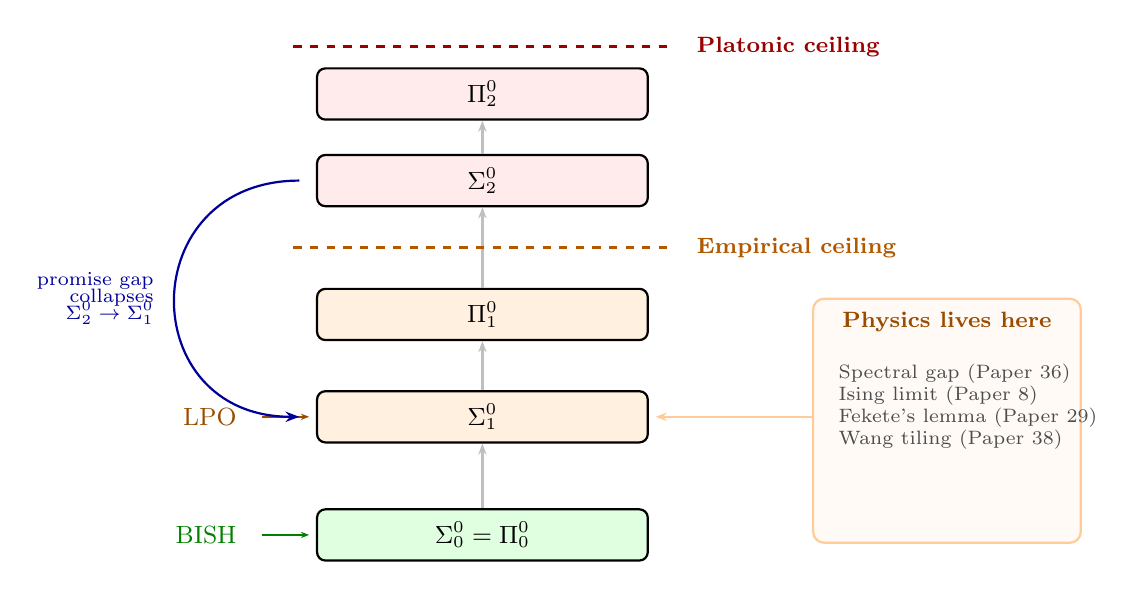
\begin{tikzpicture}[
  every node/.style={font=\small},
  level/.style={draw, thick, rounded corners=3pt, minimum width=4.2cm,
                minimum height=0.65cm, align=center},
  ceiling/.style={very thick, dashed}
]

  % --- Hierarchy levels (bottom to top) ---
  % Only levels seriously discussed in Papers 39--40:
  % Sigma^0_0 (decidable / BISH), Sigma^0_1 (LPO), Pi^0_1 (also LPO),
  % Sigma^0_2 / Pi^0_2 (Platonic ceiling).
  \node[level, fill=green!12]  (s00) at (0, 0)    {$\Sigma^0_0 = \Pi^0_0$};
  \node[level, fill=orange!12] (s01) at (0, 1.5)  {$\Sigma^0_1$};
  \node[level, fill=orange!12] (p01) at (0, 2.8)  {$\Pi^0_1$};
  \node[level, fill=red!8]     (s02) at (0, 4.5)  {$\Sigma^0_2$};
  \node[level, fill=red!8]     (p02) at (0, 5.6)  {$\Pi^0_2$};

  % --- Arrows connecting levels ---
  \draw[-{Stealth[length=4pt]}, thick, gray!50] (s00) -- (s01);
  \draw[-{Stealth[length=4pt]}, thick, gray!50] (s01) -- (p01);
  \draw[-{Stealth[length=4pt]}, thick, gray!50] (p01) -- (s02);
  \draw[-{Stealth[length=4pt]}, thick, gray!50] (s02) -- (p02);

  % --- CRM principle labels (left column) ---
  % BISH at Sigma^0_0; LPO at Sigma^0_1 (Papers 39, 40)
  \node[font=\small\bfseries, text=green!50!black, anchor=east] at (-3.0, 0)
    {$\BISH$};
  \node[font=\small\bfseries, text=orange!60!black, anchor=east] at (-3.0, 1.5)
    {$\LPO$};

  % --- Connecting arrows from CRM labels to hierarchy boxes ---
  \draw[-{Stealth[length=3pt]}, thick, green!50!black]
    (-2.8, 0) -- (-2.2, 0);
  \draw[-{Stealth[length=3pt]}, thick, orange!60!black]
    (-2.8, 1.5) -- (-2.2, 1.5);

  % === Empirical ceiling (between Pi^0_1 and Sigma^0_2) ===
  \draw[ceiling, orange!70!black]
    (-2.4, 3.65) -- (2.4, 3.65);
  \node[font=\footnotesize\bfseries, text=orange!70!black, anchor=west] at (2.6, 3.65)
    {Empirical ceiling};

  % === Platonic ceiling (above Pi^0_2) ===
  \draw[ceiling, red!60!black]
    (-2.4, 6.2) -- (2.4, 6.2);
  \node[font=\footnotesize\bfseries, text=red!60!black, anchor=west] at (2.6, 6.2)
    {Platonic ceiling};

  % --- Promise gap collapse (arrow curving on left, from Sigma^0_2 down to Sigma^0_1) ---
  \draw[-{Stealth[length=5pt]}, thick, blue!60!black]
    ([xshift=-6pt]s02.west) to[out=180, in=180, looseness=1.8]
    node[left, font=\scriptsize, text=blue!60!black, align=right, xshift=-4pt]
    {promise gap\\[-2pt]collapses\\[-2pt]$\Sigma^0_2 \to \Sigma^0_1$}
    ([xshift=-6pt]s01.west);

  % --- Physics callout (right side, spanning BISH to LPO) ---
  \draw[thick, rounded corners=4pt, orange!40, fill=orange!4]
    (4.2, -0.1) rectangle (7.6, 3.0);
  \node[font=\footnotesize\bfseries, text=orange!60!black] at (5.9, 2.7)
    {Physics lives here};
  \node[font=\scriptsize, align=left, text=gray!60!black, anchor=north west] at (4.4, 2.3)
    {Spectral gap (Paper 36)\\Ising limit (Paper 8)\\Fekete's lemma (Paper 29)\\Wang tiling (Paper 38)};
  \draw[-{Stealth[length=4pt]}, thick, orange!40] (4.2, 1.5) -- (2.2, 1.5);

\end{tikzpicture}
\caption{The two ceilings in the arithmetic hierarchy (Papers~39--40).
The \emph{empirical ceiling} at~$\Sigma^0_1$ ($\equiv \LPO$) bounds all physical
undecidability results calibrated in the series.  The \emph{Platonic ceiling}
at~$\Sigma^0_2$ bounds generic intensive observables without promise gap
(Paper~39).  The promise gap (finite experimental precision) collapses~$\Sigma^0_2$
back to~$\Sigma^0_1$, keeping empirical physics at the lower ceiling.}
\label{fig:ceilings}
\end{figure}

The promise gap is the logical mechanism separating the two ceilings.  Finite experimental precision---far from being a mere practical nuisance---is the structural feature that keeps empirical physics at~$\LPO$ rather than climbing higher in the arithmetic hierarchy.

\subsection{The conservation thesis}

Paper~40 argued that the $\BISH + \LPO$ characterization is not a coincidence of the specific theorems calibrated but reflects a structural pattern: empirical physical predictions are finite compositions of computable functions ($\BISH$), and the only idealization that exceeds finite computation is the completed limit ($\LPO$, via Bounded Monotone Convergence).  No standard physical theory invokes a higher-order quantifier alternation.

This \emph{conservation thesis} explains the uniformity of the calibrations in Papers~2--39: the logical address of each theorem is determined not by the specific physics but by the general structure of empirical prediction---computable operations plus, at most, one completed infinite limit.  The thesis is an empirical generalization, not a proved metatheorem: it could in principle be challenged by physical theories involving non-perturbative completions (instantons, resurgence, lattice strong-coupling expansions) where the relationship between finite-order computation and the completed theory is more delicate.

\subsection{Markov's Principle and physical actualisation}

Paper~43~\cite{Paper43} identified a subtler logical cost that lies \emph{below}~$\LPO$ in the hierarchy: Markov's Principle ($\MP$), which asserts that if a binary sequence is not identically zero, then it contains a~$1$ at a specific index.  $\LPO$ strictly implies~$\MP$, but not conversely; $\MP$ is independent of~$\WLPO$.

$\MP$ governs the passage from probabilistic exclusion to existential witness---the step Cournot's Principle mediates in stochastic physics.  Paper~43 exhibited three physically distinct systems that share an identical logical structure:

\begin{center}
\renewcommand{\arraystretch}{1.1}
\begin{tabular}{@{}lll@{}}
\toprule
\textbf{System} & \textbf{BISH prediction} & \textbf{MP actualisation} \\
\midrule
Radioactive decay & Detection time computable & This atom decays \\
Poincar\'e recurrence & Non-return set has measure~$0$ & This orbit returns \\
False vacuum decay & Tunnelling rate computable & Vacuum decays somewhere \\
\bottomrule
\end{tabular}
\end{center}

In each case the mathematics is entirely $\BISH$-computable, yet the physical assertion that a specific event \emph{actually occurs} requires extracting an existential witness from a~$\lnot\forall$ statement---exactly~$\MP$.  (The classification depends on interpreting physical actualization as a \emph{logical} assertion rather than a purely empirical one; different interpretations of quantum mechanics may disagree about whether this framing is appropriate.  For false vacuum decay in the context of eternal inflation, the measure problem further complicates the picture.)

$\MP$ is the unique principle where the three major constructive schools \emph{disagree}: Bishop is silent (neither accepting nor rejecting), Brouwer rejects it (along with all omniscience), and Markov's school accepts it as foundational.  This three-way split makes~$\MP$ the sharpest diagnostic for distinguishing constructive philosophies in a physical context.

The residual~$\MP$ cost reappears in the arithmetic geometry calibrations (\S\ref{sec:descent}), where the motive kills~$\LPO$ but cannot kill~$\MP$: the Diophantine search for cycle representatives or BSD generators is an~$\MP$ obstruction that no amount of algebraic structure eliminates.


%% ===================================================================
\section{The De-Omniscientizing Descent}
\label{sec:descent}
%% ===================================================================

\subsection{The pattern}

Paper~50~\cite{Paper50} identified a structural pattern, the \emph{de-omniscientizing descent}, that recurs across all five of the ``great conjectures'' calibrated in Papers~45--50.  The pattern has four stages:

\begin{enumerate}
\item \textbf{The Continuous Prison.}  Data is initially computed over a complete topological field---$\Qell$, $\Qp$, $\R$, $\C$---where testing equality requires~$\LPO$.  In this setting, even asking whether a cohomology class is zero is undecidable.

\item \textbf{The Discrete Rescue.}  Each conjecture asserts that the relevant data \emph{descends} to~$\Q$, $\Qbar$, or~$\Z$, where equality is decidable in~$\BISH$.

\item \textbf{The Geometric Mechanism.}  Descent is mediated by \emph{geometric origin}: algebraic cycles, cohomology of varieties, or other algebro-geometric structures force coefficients to be algebraic rather than transcendental.

\item \textbf{The Polarization Bifurcation.}  At finite primes ($u(\Qp) = 4$), descent proceeds purely algebraically.  At the infinite prime ($u(\R) = \infty$, so positive-definite forms exist in every dimension), the Archimedean polarization provides an additional constructive mechanism (orthogonal projection, harmonic splitting).
\end{enumerate}

\noindent After~$\LPO$ is eliminated, a Diophantine search residue ($\MP$) may remain: the motive kills~$\LPO$ but not~$\MP$.  The WMC achieves full descent ($\LPO \to \BISH$) with no~$\MP$ residue; the remaining four conjectures retain~$\MP$ from their respective search problems (cycle search, variety search, generator search).

\begin{figure}[ht]
\centering
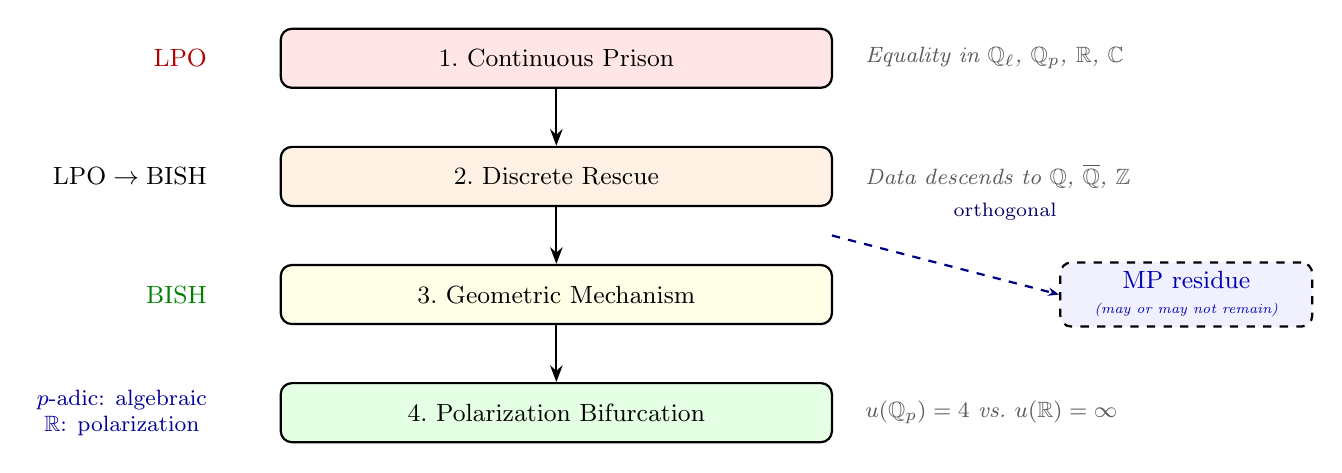
\begin{tikzpicture}[
  stage/.style={draw, rounded corners=4pt, thick, minimum width=7.0cm,
                minimum height=0.75cm, align=center, font=\small},
  arr/.style={-{Stealth[length=6pt]}, thick},
  note/.style={font=\footnotesize\itshape, text=gray!70!black, align=left},
  residual/.style={draw, rounded corners=4pt, thick, dashed,
                   minimum width=3.2cm, minimum height=0.65cm,
                   align=center, font=\small}
]
  % Main descent stages (vertical)
  \node[stage, fill=red!10]    (prison) at (0,0)
    {1.\ Continuous Prison};
  \node[stage, fill=orange!10] (rescue) at (0,-1.5)
    {2.\ Discrete Rescue};
  \node[stage, fill=yellow!10] (geom)   at (0,-3.0)
    {3.\ Geometric Mechanism};
  \node[stage, fill=green!10]  (polar)  at (0,-4.5)
    {4.\ Polarization Bifurcation};

  % Arrows
  \draw[arr] (prison)  -- (rescue);
  \draw[arr] (rescue)  -- (geom);
  \draw[arr] (geom)    -- (polar);

  % Level labels on left
  \node[left=0.8cm of prison,  font=\small\bfseries, text=red!70!black]  {$\LPO$};
  \node[left=0.8cm of rescue,  font=\small]  {$\LPO \to \BISH$};
  \node[left=0.8cm of geom,    font=\small\bfseries, text=green!50!black]  {$\BISH$};

  % Bifurcation labels for stage 4
  \node[font=\footnotesize, text=blue!60!black, align=center,
        left=0.8cm of polar] {$p$-adic: algebraic\\$\R$: polarization};

  % Annotations on right (kept short to leave room for MP box)
  \node[note, anchor=west] at (3.8, 0)    {Equality in $\Qell$, $\Qp$, $\R$, $\C$};
  \node[note, anchor=west] at (3.8,-1.5)  {Data descends to $\Q$, $\Qbar$, $\Z$};
  \node[note, anchor=west] at (3.8,-4.5)  {$u(\Qp)=4$ vs.\ $u(\R)=\infty$};

  % MP residue: logically appears after LPO is killed (between stages 2--3)
  % Placed far right to avoid annotation overlap
  \node[residual, fill=blue!6, text=blue!70!black, align=center] (mp) at (8.0,-3.0)
    {$\MP$ residue\\[-2pt]{\tiny\itshape (may or may not remain)}};
  % Dashed arrow: right from descent column at stage-2/3 boundary
  \draw[-{Stealth[length=4pt]}, dashed, blue!50!black, thick]
    (3.5,-2.25) -- (mp.west);
  \node[font=\scriptsize, text=blue!40!black, above=2pt] at (5.7,-2.25) {orthogonal};
\end{tikzpicture}
\caption{The de-omniscientizing descent (Paper~50).
Data trapped in a complete field ($\LPO$) descends to an algebraic field ($\BISH$)
via geometric origin; the polarization bifurcation distinguishes the Archimedean
and $p$-adic mechanisms.  An $\MP$ residue (dashed) may remain as an orthogonal
Diophantine search cost; the WMC has none, while the other four conjectures
retain~$\MP$.  The motive kills~$\LPO$ but not~$\MP$.}
\label{fig:descent}
\end{figure}

\subsection{The five conjectures}

Paper~50~\cite{Paper50} calibrated five major conjectures against this pattern (Figure~\ref{fig:descent}):

\begin{description}[leftmargin=2em]
\item[Weight-Monodromy] (Paper~45).  The spectral sequence degenerating at~$E_2$ asserts that eigenvalues of Frobenius on $\ell$-adic cohomology are algebraic.  Abstract strength:~$\LPO$ (equality in~$\Qell$).  Geometric strength:~$\BISH$ (eigenvalues in~$\Qbar$, checkable by minimal polynomials).

\item[Tate Conjecture] (Paper~46).  The $\ell$-adic Galois-fixed subspace of cohomology is spanned by algebraic cycles.  This forces eigenvectors (not just eigenvalues) to descend to~$\Qbar$.  Residual:~$\MP$ (searching for the cycle representatives).

\item[Fontaine-Mazur] (Paper~47).  A $p$-adic Galois representation that is de~Rham comes from the \'etale cohomology of an algebraic variety.  The abstract~$\LPO$ cost arises from zero-testing in~$p$-adic cohomology; the conjecture asserts that geometric origin forces the relevant structure to descend to algebraic de~Rham cohomology, where the cost reduces.  (The de~Rham condition itself can in principle be checked via the Colmez--Fontaine criterion---admissibility of the filtered $\varphi$-module---so it is closer to decidable than the general representation-theoretic question.)  The preliminary CRM reading is that geometric origin eliminates the $\LPO$ component; the full calibration awaits Paper~47.

\item[Birch--Swinnerton-Dyer] (Paper~48, implemented in Paper~51).  The rank of~$E(\Q)$ equals the order of vanishing of~$L(E, s)$ at~$s = 1$.  For rank~1, the Gross--Zagier formula and the positive-definite N\'eron--Tate height convert the generator search from~$\MP$ (unbounded) to~$\BISH$ (bounded Finset of size~$O(B^2)$).

\item[Hodge Conjecture] (Paper~49).  Every Hodge class is algebraic.  This is the nexus where both the~$\LPO$ and~$\MP$ obstructions interact: the Hodge filtration provides an Archimedean splitting (since~$u(\R) = \infty$, positive-definite forms exist in every dimension), but the algebraicity question remains.
\end{description}

\subsection{The motive as LPO-killer}

The uniform pattern across all five conjectures leads to a precise characterization.  Paper~50 proposed that Grothendieck's category of numerical motives is characterized by three axioms:
\begin{enumerate}[label=(\roman*)]
\item \textbf{Decidable equality} on morphism spaces (Standard Conjecture~D---\emph{conjectural} in general, known for abelian varieties by Lieberman~\cite{Lieberman});
\item \textbf{Algebraic spectrum}: eigenvalues are algebraic, characteristic polynomials are $\ell$-independent (\emph{largely a theorem}: algebraicity of eigenvalues is Deligne's theorem (Weil~II); $\ell$-independence is known in many cases but not in full generality);
\item \textbf{Archimedean polarization}: a positive-definite bilinear form exists (\emph{a theorem} for projective varieties over~$\R$ by the Hodge index theorem; the axiom concerns its availability in the abstract motive category).
\end{enumerate}

These axioms encode exactly the de-omniscientizing descent: Axiom~(i) is the target ($\LPO$ eliminated); Axiom~(ii) provides the algebraic rescue; Axiom~(iii) provides the computational mechanism (positive-definiteness enables Gram--Schmidt, projection, and norm comparison).  The three axioms thus span a range from open conjecture to established theorem, and the DPT framework is conditional primarily on~(i).

The motive thus functions as a \emph{decidability certificate}: an algebraic structure that guarantees the computability of cohomological data.  It kills~$\LPO$---the topological undecidability---but cannot kill~$\MP$---the Diophantine search.  This is the precise sense in which the Standard Conjectures are decidability axioms.

\subsection{The polarization bifurcation}

The third axiom (Archimedean polarization) has a distinguished role.  Over~$\R$, the $u$-invariant is $u(\R) = \infty$: positive-definite (anisotropic) forms exist in every dimension.  Over~$\Qp$, the $u$-invariant is~$u(\Qp) = 4$: no anisotropic form of dimension~$> 4$ exists.  This bifurcation becomes relevant in higher dimensions, where the height pairing on an abelian variety of dimension~$g$ is a quadratic form in~$g$ variables: for~$g \ge 5$, the $p$-adic pairing cannot be positive-definite.

For the BSD rank-1 case (Paper~51), the mechanism is different but the conclusion is the same.  The N\'eron--Tate canonical height~$\hat{h}$ on an elliptic curve~$E/\Q$ is positive-definite at the Archimedean place ($\hat{h}(P) > 0$ for all~$P \ne O$).  The $p$-adic height pairing~$\hat{h}_p$, by contrast, can vanish on non-torsion points.  This failure stems from the structure of $p$-adic integration: the $p$-adic height depends on a choice of splitting of the Hodge filtration (via the Iwasawa logarithm), and different choices can produce degenerate pairings.  The Archimedean metric is not merely convenient---it is the \emph{unique} topological modality enabling the~$\MP \to \BISH$ reduction.


%% ===================================================================
\section{The Dimension-4 Wall}
\label{sec:wall}
%% ===================================================================

\subsection{Two roads to the same wall}

Papers~50, 52, and~53 approach the decidability boundary for abelian varieties from three different angles.  All three converge on the same answer: dimension~4.

\begin{description}[leftmargin=2em]
\item[Paper~50: the CM bridge.] The CM (complex multiplication) structure on an abelian variety~$X$ provides an explicit basis for the cycle algebra and computable intersection numbers.  For CM abelian varieties of dimension~$g \le 3$, this yields a verified decidability oracle.  At~$g = 4$, exotic Weil classes---algebraic Hodge classes outside the Lefschetz ring---appear.  The CM bridge cannot access them: the exotic classes escape the CM structure.

\item[Paper~52: the specialization transfer.] Decidability of numerical equivalence over~$\Q$ can be transferred from decidability over finite fields~$\Fq$ via specialization, provided the Lefschetz ring generates all algebraic classes.  For~$g \le 3$, it does: Moonen and Zarhin~\cite{MoonenZarhin1999} showed that all Hodge classes on abelian varieties of dimension~$\le 3$ lie in the Lefschetz ring.  At~$g = 4$, exotic Tate classes appear over~$\Fq$ that lie outside the Lefschetz ring, and the transfer fails.

\item[Paper~53: the computation.] The exotic Weil class on Milne's CM abelian fourfold~$A \times B$ (with Hermitian form~$H = \mathrm{diag}(1, -1, -1, 1)$ over~$\Q(\sqrt{-3})$) has self-intersection:
\[
\deg(w \cdot w) = 7 > 0.
\]
This is machine-verified arithmetic---no custom axioms, no~\texttt{sorry}---confirming that the exotic class satisfies the Hodge--Riemann bilinear relations.
\end{description}

\subsection{Visibility versus pathology}

The convergence of three independent approaches on the same dimension demands explanation.  The key insight, implicit in Milne's original example~\cite{Milne2001} and van~Geemen's framework~\cite{vanGeemenCIME,vanGeemen2022}, and made computationally explicit in Paper~53, is that the dimension-4 obstruction is a \emph{visibility problem}, not a \emph{pathology}.

The exotic Weil class is:
\begin{itemize}[nosep]
\item \emph{Algebraic}---proved by Schoen~\cite{Schoen} via the order-3 automorphism of the CM elliptic curve.
\item \emph{Numerically well-behaved}---self-intersection~$\deg(w \cdot w) = 7 > 0$, satisfying the Hodge--Riemann bilinear relations.
\item \emph{Computationally accessible}---the cross-pairing formula, the trace, and the sign are all verified by the Lean kernel as pure arithmetic.
\end{itemize}

But it is \emph{invisible} to the Lefschetz ring---the subring of the cohomology algebra generated by the hyperplane class under the Lefschetz operators~$L$ and~$\Lambda$.  The decidability oracle uses the Lefschetz ring as its ``eye'': it can see and compare anything in this ring, but the exotic class lies outside.

The analogy is to a measuring instrument with a blind spot.  The instrument is not broken---it measures everything in its range correctly.  But its range does not cover the full space, and the uncovered region contains genuine, healthy objects.

\subsection{Dimension~$\ge 5$: the wall gets worse}

At dimension~5 and above, the situation deteriorates further.  Agugliaro~(2025,~\cite{Agugliaro2025}) constructs exotic Tate classes over finite fields that are \emph{non-liftable} to characteristic~0.  This means that not only can the decidability oracle not see these classes---they cannot even be compared to their characteristic-0 analogues, because no such analogues exist.

The decidability landscape is therefore stratified (Figure~\ref{fig:wall}):

\begin{figure}[ht]
\centering
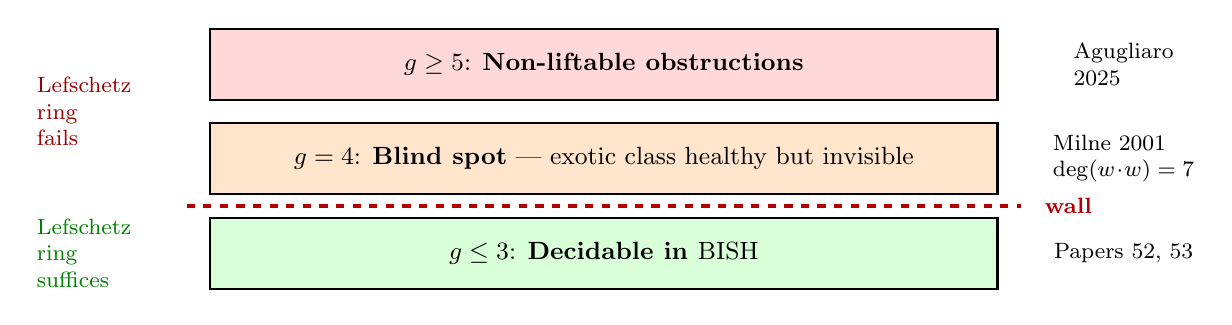
\begin{tikzpicture}[
  layer/.style={draw, thick, minimum height=0.9cm, align=center, font=\small},
  note/.style={font=\footnotesize, align=left}
]
  % Layers (bottom to top = dimension increasing)
  \node[layer, fill=green!15, minimum width=10cm]
    (low)  at (0,0) {$g \le 3$: \textbf{Decidable in $\BISH$}};
  \node[layer, fill=orange!20, minimum width=10cm]
    (four) at (0,1.2) {$g = 4$: \textbf{Blind spot} --- exotic class healthy but invisible};
  \node[layer, fill=red!15, minimum width=10cm]
    (high) at (0,2.4) {$g \ge 5$: \textbf{Non-liftable obstructions}};

  % Wall marker
  \draw[very thick, red!70!black, dashed]
    (-5.3,0.6) -- (5.3,0.6);
  \node[font=\footnotesize\bfseries, text=red!70!black] at (5.9,0.6) {wall};

  % Left annotations
  \node[note, text=green!50!black] at (-6.6,0)
    {Lefschetz\\ring\\suffices};
  \node[note, text=red!60!black] at (-6.6,1.8)
    {Lefschetz\\ring\\fails};

  % Right annotations
  \node[note] at (6.6,0)   {Papers 52, 53};
  \node[note] at (6.6,1.2) {Milne 2001\\$\deg(w\!\cdot\! w)=7$};
  \node[note] at (6.6,2.4) {Agugliaro\\2025};
\end{tikzpicture}
\caption{The dimension-4 wall.  Below the wall, the Lefschetz ring generates
all algebraic classes and numerical equivalence is decidable.  At~$g=4$,
exotic Weil classes escape the Lefschetz ring (a visibility failure, not a
pathology).  At~$g \ge 5$, non-liftable Tate classes appear.}
\label{fig:wall}
\end{figure}


%% ===================================================================
\section{What This Says for Physics}
\label{sec:physics}
%% ===================================================================

\subsection{The logical cost of physical theorems}

Section~\ref{sec:constitution} advanced the thesis that empirical physics requires exactly $\BISH + \LPO$, with the completed infinite limit as the sole source of undecidability.  For a physicist, the message is: everything measurable in a finite laboratory is constructive ($\BISH$); the idealization to infinite volume or completed limits carries a logical cost ($\LPO$); and the passage from probabilistic prediction to individual-event assertion carries a further cost ($\MP$).  These are not artifacts of formalism---they track the difference between what a finite machine can compute and what requires idealized infinite operations.

\subsection{Dimension~4 and spacetime}

The dimension-4 boundary discovered in Papers~50--53 invites a physics reading.  Spacetime is four-dimensional, and the decidability boundary for abelian varieties falls at exactly dimension~4.  Is this a coincidence?

We urge caution.  The dimension in question is the dimension of the abelian variety as a complex manifold, not the dimension of spacetime.  The exotic Weil classes are cohomological objects on algebraic varieties, not physical fields.  The connection, if any, would have to pass through deep and currently speculative links between motives and quantum field theory (cf.\ Kontsevich--Zagier on periods, or Connes--Marcolli on the cosmic Galois group).

What we \emph{can} say is this: the logical structure of arithmetic geometry changes qualitatively at dimension~4, and any physical theory that depends on the arithmetic of four-dimensional varieties---such as compactifications in string theory or period integrals in gauge theory---inherits this qualitative change.  Whether this has physical consequences remains an open question.

\subsection{The Archimedean metric in physics}

Paper~51 showed that the positive-definiteness of the N\'eron--Tate height---a consequence of the Archimedean metric on~$\R$---is the exact modality converting the BSD generator search from unbounded ($\MP$) to bounded ($\BISH$).  The $p$-adic analogue fails because the $p$-adic metric is not positive-definite in the relevant sense.

For physics, this means: the real number line is computationally privileged.  Its completeness and ordering---which give rise to positive-definite inner products, norms, and Hilbert space structure---are not just convenient but \emph{indispensable} for reducing computational problems from infinite search to finite verification.  The ubiquity of Hilbert space in quantum mechanics is, from the CRM perspective, a manifestation of the Archimedean metric's computational power.


%% ===================================================================
\section{What This Says for Philosophy}
\label{sec:philosophy}
%% ===================================================================

\subsection{Beyond decidable and undecidable}

Classical logic offers a binary classification: a mathematical question is either decidable or undecidable.  G\"odel's incompleteness theorems and Turing's halting problem established this boundary as fundamental.  Intuitionistic logic~\cite{Dummett2000} refines this picture, but its implications for specific mathematical practice have remained largely unexplored.

CRM reveals a much finer landscape.  Between ``decidable'' and ``undecidable'' lie multiple distinct levels, each corresponding to a different kind of computational resource:

\begin{itemize}[nosep]
\item $\BISH$: finite exact computation with no oracles.
\item $\BISH + \WLPO$: computation with access to a ``weak oracle'' that detects whether a sequence is identically zero (but cannot find a nonzero element).
\item $\BISH + \LPO$: computation with a ``strong oracle'' that both detects and locates nonzero elements.
\item $\CLASS$: full classical reasoning (unrestricted excluded middle).
\end{itemize}

The program's calibrations show that theorems \emph{naturally distribute} across these levels.  The bidual gap sits at~$\WLPO$, not higher and not lower.  The thermodynamic limit sits at~$\LPO$, not higher and not lower.  These are not artifacts of proof technique---they are \emph{equivalences}: the mathematical theorem is logically interchangeable with the principle.

This distribution suggests that the logical hierarchy is a natural feature of mathematical reality, not an artificial imposition.  Theorems have logical addresses, and finding those addresses reveals computational structure invisible to classical analysis.

\subsection{The absence of G\"odel on the geometric side}

Uncomputability (Turing~1936), incompleteness (G\"odel~1931), and constructive undecidability (CRM) are three manifestations of the same diagonal phenomenon, but at different levels.  Uncomputability limits what \emph{functions} machines can compute; incompleteness limits what \emph{truths} a formal system can prove; CRM undecidability limits which \emph{disjunctions}~$P \lor \neg P$ hold constructively.  The logical landscape is:
\[
  \BISH \;\subset\; \BISH + \LPO \;=\; \text{Turing ceiling} \;\subset\; \CLASS \;\supset\; \text{G\"odel ceiling},
\]
where $\BISH + \LPO$ is the join of the incomparable principles $\WLPO$ and $\MP$, corresponding respectively to the $\Pi^0_1$ oracle (deciding whether a binary sequence is identically zero) and the extraction of witnesses from double negations ($\lnot\lnot\exists n \to \exists n$).  $\LPO$ itself is the~$\Sigma^0_1$ oracle: deciding whether a binary sequence contains a~$1$.

A striking feature of the program is that the geometric side---motives, cycle class maps, intersection pairings---\emph{never reaches the G\"odel level}.  G\"odel incompleteness requires a formal system strong enough to encode its own provability predicate via self-referential arithmetic.  The objects manipulated by the motive are finite-dimensional: cohomology groups, algebraic cycles of bounded degree, matrices with algebraic entries.  There is no self-referential encoding, hence no diagonal argument, hence no incompleteness phenomenon.

The analytic side (physics) saturates at~$\LPO$, the Turing ceiling: it needs the ability to decide convergence of specific infinite sequences, but never requires the full power of classical logic.  The geometric rescue then \emph{descends} from~$\LPO$ to~$\MP$, replacing the infinite oracle with finitary algebraic verification.  The residual~$\MP$ cost---the Diophantine search for an explicit witness---is a computational task, not a logical one.

This architecture means the program moves \emph{away from} G\"odel, not toward it.  The motive does not encounter incompleteness because it operates in finitary linear algebra; it does not encounter uncomputability because the algebraic spectrum (DPT Axiom~2) ensures all eigenvalues are algebraic numbers admitting effective arithmetic.  The only place G\"odel could lurk is in the \emph{meta-question} of whether Standard Conjecture~D is itself provable in~ZFC---but this lies outside the framework, not inside it.

Paper~55~\cite{Paper55} makes this remark precise: Conjecture~D is an arithmetical sentence ($\Pi^0_2$ in characteristic~$0$, $\Pi^0_3$ in positive characteristic due to $\ell$-adic approximation), hence absolute between all transitive models of~ZFC by Shoenfield's absoluteness theorem.  Cohen forcing and large cardinal axioms cannot affect its truth value.  The residual possibility---G\"odel independence, where Conjecture~D is true but unprovable---remains open but is unlikely given the precedent from algebraic geometry.  The CRM program's conditional architecture insulates all calibration results from both modes of independence.

\subsection{The Kantian reading}

The dimension-4 obstruction admits a reading through Kant's epistemology.  In the \emph{Critique of Pure Reason}, Kant distinguished between \emph{things in themselves} (Dinge an sich) and \emph{things as they appear to us} (Erscheinungen), mediated by the \emph{categories of understanding}---the conceptual apparatus through which the mind organizes experience.

In the CRM setting, the Lefschetz ring plays the role of a category of understanding.  It is the conceptual apparatus through which the decidability oracle ``experiences'' the cohomology algebra.  Everything within the Lefschetz ring is accessible: the oracle can see it, compare it, decide equality.

The exotic Weil class exists ``in itself''---it is algebraic (Schoen), has positive self-intersection ($\deg(w \cdot w) = 7$), and satisfies the Hodge--Riemann relations.  But it does not exist ``for the oracle''---it lies outside the Lefschetz ring, invisible to the decidability machinery.

The gap between the class's existence and its accessibility is \emph{intrinsic to the dimension}: it does not appear at~$g \le 3$ and cannot be removed at~$g = 4$ without importing non-constructive input (Schoen's algebraicity theorem, which uses non-constructive methods).  This is not a technical limitation to be overcome by better algorithms, but a structural feature of the mathematical landscape.

Whether one accepts the Kantian framing or not, the phenomenon is real: mathematical objects can be well-defined, well-behaved, and computationally accessible \emph{in parts}, while remaining invisible to the standard computational apparatus \emph{as a whole}.

\subsection{Logical versus geometric obstructions}

The distinction between logical and geometric obstructions is, we believe, philosophically novel.

A \emph{logical} obstruction means: you cannot avoid using an omniscience principle.  The theorem genuinely requires the ability to survey an infinite domain.  Papers~2, 7, and~8 demonstrate this for functional analysis and statistical physics.  The obstruction is in the \emph{logic}---the structure of the proof, not the structure of the objects.

A \emph{geometric} obstruction means: the objects are computationally well-behaved, but the standard tools cannot see all of them.  Papers~52 and~53 demonstrate this for abelian fourfolds.  The obstruction is in the \emph{geometry}---the relationship between the objects and the instruments used to study them.

This distinction matters because it implies that the limits of mathematical computation are not monolithic.  Some limits are about \emph{logic} (what can be decided in principle); others are about \emph{vision} (what the available tools can access).  The second kind might, in principle, be overcome by new tools---but Paper~53's computation shows that for the Lefschetz-based approach, the dimension-4 limit is sharp.

\subsection{Three convergent traditions}

The program draws an unexpected connection between Brouwer's intuitionism (Fan Theorem, Paper~23), Bishop's constructivism~\cite{Bishop1967} ($\BISH$ as the base of the hierarchy), and Grothendieck's motives~\cite{Grothendieck1969} (the geometric objects).  These traditions were developed independently, but the CRM atlas reveals that they converge on a common question: \emph{what can be computed about the geometry of algebraic varieties?}  The motive as decidability certificate (\S\ref{sec:descent}) is precisely the point of convergence.


%% ===================================================================
\section{What This Says for Arithmetic Geometry}
\label{sec:ag}
%% ===================================================================

\subsection{Standard Conjecture~D as decidability axiom}

Paper~50, Theorem~C, established that Standard Conjecture~D is a decidability axiom for the motive category: it ensures that the \emph{equivalence relation} defining the morphism spaces is decidable.

Precisely: homological equivalence is tested in~$\Qell$-cohomology, where zero-testing requires~$\LPO$.  Numerical equivalence is tested by intersection numbers, which are integers---decidable by finite computation.  Conjecture~D asserts that these two notions coincide, so the~$\LPO$-level question reduces to a~$\BISH$-level one.  This gives decidability of the \emph{equivalence relation}, not effective computability of the full morphism spaces.  The latter requires additional input---an explicit basis for the Chow group or the numerical equivalence classes---which Conjecture~D alone does not provide.  (In the CM case of Paper~53, the CM endomorphism ring supplies this additional input.)

For abelian varieties, Conjecture~D is known (Lieberman~\cite{Lieberman}).  Paper~53 exploits this, together with the explicit CM structure, to build a verified decidability oracle for the~13 CM elliptic curves over~$\Q$ with class number~1.

\subsection{The CM rescue}

Paper~50, Theorem~E, and Paper~53, Theorem~A, demonstrated that CM abelian varieties provide an \emph{unconditional} decidability result.  No Standard Conjecture is assumed.  The CM endomorphism ring provides an explicit basis for the cycle algebra, and the norm formula provides computable intersection numbers.  The result is a verified decision procedure that takes two algebraic cycles and returns a Boolean, with machine-checked correctness.

This is the CRM ideal realized: a theorem of arithmetic geometry that is not merely true but \emph{computationally effective}, with every step verified by a proof assistant.  The 13~CM elliptic curves serve as test cases, but the architecture extends in principle to any abelian variety with sufficiently explicit endomorphism structure.

\subsection{The Hodge conjecture as visibility hypothesis}

The exotic Weil class on a CM abelian fourfold is algebraic by Schoen's theorem~\cite{Schoen}.  From the CRM perspective, Schoen's result is a \emph{visibility theorem}: it asserts that the exotic class, although invisible to the Lefschetz ring, is genuinely algebraic---it can be represented by an algebraic cycle.

The Hodge conjecture, more broadly, is a visibility hypothesis: it asserts that every Hodge class (a class that ``looks algebraic'' from the Hodge-theoretic perspective) actually \emph{is} algebraic.  In CRM terms, this would extend the decidability of the Lefschetz ring to the full space of Hodge classes.  (We note that the integral Hodge conjecture fails---Atiyah and Hirzebruch constructed counterexamples---and the Hodge conjecture fails for K\"ahler manifolds by work of Voisin.  The ``visibility'' interpretation applies specifically to the rational Hodge conjecture for projective varieties.)

The catch is that Schoen's proof is non-constructive---it uses the order-3 automorphism and a counting argument, not an explicit cycle construction.  A constructive proof would convert the visibility theorem into a decidability extension.  Whether such a constructive proof exists is one of the open questions highlighted in Paper~53.

\subsection{Relationship to classical decidability in algebraic geometry}

The CRM notion of decidability---whether a theorem can be proved without omniscience principles---is related to, but distinct from, the classical computability-theoretic notion---whether there exists an algorithm.  The extensive literature on decidability and undecidability in algebraic geometry~\cite{Poonen2008,Mazur1994} addresses the latter: Poonen's work on the undecidability of Hilbert's 10th problem over~$\Q$ and function fields, and Koenigsmann's definability of~$\Z$ in~$\Q$, concern the existence of algorithms for Diophantine problems.  These are precisely the kind of ``Diophantine obstructions'' that appear in the CRM framework as~$\MP$ residuals.

The CRM program adds a finer classification: within the realm of algorithmically solvable problems, it distinguishes between those requiring an oracle ($\LPO$), those requiring witness extraction ($\MP$), and those constructively decidable ($\BISH$).  Classical undecidability results (such as the undecidability of the isomorphism problem for algebraic varieties) sit above the CRM hierarchy entirely---they are problems where no algorithm exists, regardless of logical strength.  A systematic comparison of the CRM hierarchy with the classical decidability landscape in arithmetic geometry is an important direction for future work.

\subsection{Open questions for arithmetic geometry}

\begin{enumerate}
\item Can the DPT framework be extended to dimension~4 by incorporating the Hodge conjecture (for Weil-type fourfolds) as an additional axiom?  What logical strength would such an extension require?

\item Is there a constructive proof of Schoen's algebraicity result for exotic Weil classes?  A constructive proof would immediately extend the decidability oracle to dimension~4.

\item Does the visibility obstruction at dimension~4 manifest differently in motivic cohomology or derived categories, where the Lefschetz ring plays a less central role?

\item Can the cross-pairing formula of Paper~53 be derived directly from van~Geemen's framework and formalized as a Lean theorem, replacing the documentary axioms?
\end{enumerate}


%% ===================================================================
\section{The Series in Retrospect}
\label{sec:retrospect}
%% ===================================================================

\subsection{Lessons and surprises}

The program began with Banach spaces (Paper~2) and ended with motives (Paper~53), traversing functional analysis, quantum mechanics, statistical physics, optimization, foundations, and arithmetic geometry.  Two findings were genuinely unexpected.  First, the transition from logical to geometric obstructions: the program began expecting all obstructions to be omniscience principles, and the emergence of a structurally different kind (geometric visibility) required new conceptual vocabulary.  Second, the sharpness of the dimension-4 boundary: that two independent proof strategies both fail at exactly dimension~4, for structurally related but technically distinct reasons, suggests the boundary is a natural feature of the mathematical landscape.

\subsection{Methodology}

Paper~10~\cite{Paper10} established the methodological framework for the series.  The key principles are:

\begin{itemize}[nosep]
\item \textbf{Constructive stratification by proof content.}  The CRM classification of a theorem is determined by the structure of its proof (explicit witnesses, no omniscience hypotheses), not by the output of Lean's \texttt{\#print axioms} command.  Lean's~$\R$ (a Cauchy completion) pervasively introduces \texttt{Classical.choice} as an infrastructure artifact; all theorems over~$\R$ carry it.  This does not affect the CRM classification.

\item \textbf{Three certification levels.}  Mechanically certified (full CRM over Mathlib, zero \texttt{sorry}); structurally verified (bridge axioms, assembly verified in Lean); intentional classical content (meta-classical reasoning for object-level BISH equivalences).

\item \textbf{Classical metatheory.}  Following the standard methodology of reverse mathematics (Friedman, Simpson~\cite{Simpson2009}), the CRM program uses classical metatheory to establish object-level constructive results.  This is not a compromise but the standard practice: $\mathrm{RCA}_0$-based reverse mathematics also operates within~$\mathrm{ZFC}$.
\end{itemize}

\subsection{What remains open}

Beyond the specific open questions raised in each paper, three broad directions remain:

\begin{enumerate}
\item \textbf{The five conjectures themselves.}  The CRM calibrations are conditional: they characterize the logical content of the conjectures, not their truth.  If the Hodge conjecture is false, the CRM calibration still stands (it characterizes what the conjecture \emph{would} achieve logically).

\item \textbf{Realizability and categorical models.}  The CRM hierarchy could be modeled in a realizability topos, making the logical levels into mathematical objects.  This would allow the calibration results to be stated as theorems about specific toposes, not just about proof-theoretic principles.

\item \textbf{Formalization coverage.}  Twelve papers carry complete Lean~4 formalizations.  Extending this to the remaining calibrations---particularly Papers~46--49 (Tate, Fontaine-Mazur, BSD atlas, Hodge)---is a substantial but achievable goal.
\end{enumerate}


%% ===================================================================
\section{Conclusion}
\label{sec:conclusion}
%% ===================================================================

The constructive reverse mathematics program, across 53~papers and one synthesis, has pursued a single thesis: every major mathematical theorem has a natural logical address, and finding that address reveals computational structure invisible to classical analysis.

The thesis has held up.  The bidual gap lives at~$\WLPO$.  The thermodynamic limit lives at~$\LPO$.  The preparation uncertainty principle lives at~$\BISH$.  The five great conjectures of arithmetic geometry exhibit a uniform de-omniscientizing descent from~$\LPO$ to~$\BISH$, mediated by the motive.  And at dimension~4, where logic meets geometry, the program discovers a new kind of obstruction: the exotic Weil class is healthy, computable in parts, but invisible to the Lefschetz ring that the decidability oracle uses as its eye.

The final calibration of the series is thus a boundary marker: the dimension-4 wall, where two independent proof strategies fail for structurally related reasons, and where a machine-verified computation ($\deg(w \cdot w) = 7 > 0$) confirms that the wall is real.  Beyond this wall, the relationship between decidability and geometry remains to be explored.

\medskip
The complete Lean~4 source code for all formalized papers in the series is available at Zenodo (individual DOIs cited in the respective papers).


%% ===================================================================
\section*{Acknowledgments}
\addcontentsline{toc}{section}{Acknowledgments}
%% ===================================================================

The constructive reverse mathematics program owes its foundations to the work of Bishop~\cite{Bishop1967}, Bridges and Richman~\cite{BridgesRichman1987}, and Ishihara~\cite{Ishihara2006}, who developed the framework that makes these calibrations possible.  The Mathlib contributors built the Lean~4 infrastructure underlying all formalizations.  The arithmetic geometry calibrations draw heavily on the work of Grothendieck, Lieberman, Milne, Schoen, and van~Geemen.

This synthesis was produced using AI text generation (Claude, Opus~4.6) under human direction.  The author is a practicing cardiologist rather than a professional logician or arithmetic geometer; all mathematical claims should be evaluated on their formal content.  The results and interpretations presented here are preliminary, and domain experts may disagree with the CRM readings of specific theorems.  We welcome constructive feedback from all three communities addressed in this work.


%% ===================================================================
\begin{thebibliography}{30}
%% ===================================================================

\bibitem{Agugliaro2025}
A.~Agugliaro.
Non-liftable exotic Tate classes on abelian varieties over finite fields.
\textit{arXiv}:2510.21562, 2025.

\bibitem{Bishop1967}
E.~Bishop.
\textit{Foundations of Constructive Analysis}.
McGraw-Hill, 1967.

\bibitem{BridgesRichman1987}
D.~Bridges and F.~Richman.
\textit{Varieties of Constructive Mathematics}.
LMS Lecture Note Series 97. Cambridge University Press, 1987.

\bibitem{CubittPerezGarciaWolf2015}
T.\,S.~Cubitt, D.~Perez-Garcia, and M.\,M.~Wolf.
Undecidability of the spectral gap.
\textit{Nature}, 528:207--211, 2015.

\bibitem{Dummett2000}
M.~Dummett.
\textit{Elements of Intuitionism}.
Oxford Logic Guides 39. Oxford University Press, 2nd edition, 2000.

\bibitem{Grothendieck1969}
A.~Grothendieck.
Standard conjectures on algebraic cycles.
In \textit{Algebraic Geometry (Bombay, 1968)}, pages 193--199. Oxford University Press, 1969.

\bibitem{Lieberman}
D.\,I.~Lieberman.
Numerical and homological equivalence of algebraic cycles on Hodge manifolds.
\textit{Amer.\ J.\ Math.}, 90:366--374, 1968.

\bibitem{Milne2001}
J.\,S.~Milne.
The Tate conjecture for certain abelian varieties over finite fields.
\textit{Acta Arith.}, 100:135--166, 2001.

\bibitem{MoonenZarhin1999}
B.~Moonen and Y.\,G.~Zarhin.
Hodge classes on abelian varieties of low dimension.
\textit{Math.\ Ann.}, 315:711--733, 1999.

\bibitem{Paper2}
P.\,C.\,K.~Lee.
WLPO and the bidual gap in constructive Banach space theory (Paper~2, CRM series).
\textit{Zenodo}, 2025.

\bibitem{Paper6}
P.\,C.\,K.~Lee.
The Heisenberg uncertainty principle in constructive reverse mathematics (Paper~6, CRM series).
\textit{Zenodo}, 2025.

\bibitem{Paper7}
P.\,C.\,K.~Lee.
Reflexive Banach spaces and WLPO dispensability (Paper~7, CRM series).
\textit{Zenodo}, 2025.

\bibitem{Paper8}
P.\,C.\,K.~Lee.
LPO dispensability in the 1D Ising model (Paper~8, CRM series).
\textit{Zenodo}, 2025.

\bibitem{Paper10}
P.\,C.\,K.~Lee.
Certification methodology for constructive reverse mathematics in a classical metatheory (Paper~10, CRM series).
\textit{Zenodo}, 2025.

\bibitem{Paper23}
P.\,C.\,K.~Lee.
The Fan Theorem and compact optimization (Paper~23, CRM series).
\textit{Zenodo}, 2025.

\bibitem{Paper28}
P.\,C.\,K.~Lee.
Newton versus Lagrange: BISH--FT stratification of classical mechanics (Paper~28, CRM series).
\textit{Zenodo}, 2025.

\bibitem{Paper29}
P.\,C.\,K.~Lee.
Fekete's Subadditive Lemma is equivalent to LPO (Paper~29, CRM series).
\textit{Zenodo}, 2025.

\bibitem{Paper30}
P.\,C.\,K.~Lee.
Fan Theorem dispensability for physical calibrations (Paper~30, CRM series).
\textit{Zenodo}, 2025.

\bibitem{Paper31}
P.\,C.\,K.~Lee.
Dependent Choice dispensability for physical calibrations (Paper~31, CRM series).
\textit{Zenodo}, 2025.

\bibitem{Paper36}
P.\,C.\,K.~Lee.
The spectral gap problem is LPO-equivalent (Paper~36, CRM series).
\textit{Zenodo}, 2025.

\bibitem{Paper37}
P.\,C.\,K.~Lee.
The undecidability landscape of physics at LPO (Paper~37, CRM series).
\textit{Zenodo}, 2025.

\bibitem{Paper38}
P.\,C.\,K.~Lee.
Wang tiling and the LPO-equivalence of combinatorial undecidability (Paper~38, CRM series).
\textit{Zenodo}, 2025.

\bibitem{Paper40}
P.\,C.\,K.~Lee.
The logical constitution of physical reality: a constructive reverse mathematics monograph (Paper~40, CRM series).
\textit{Zenodo}, 2025.

\bibitem{Paper43}
P.\,C.\,K.~Lee.
What the ceiling means: constructive schools, physical actualisation, and the fine structure of $\mathrm{BISH} + \mathrm{LPO}$ (Paper~43, CRM series).
\textit{Zenodo}, 2025.

\bibitem{Paper45}
P.\,C.\,K.~Lee.
The Weight-Monodromy Conjecture and LPO: a constructive calibration of spectral sequence degeneration via de-omniscientizing descent (Paper~45, CRM series).
\textit{Zenodo}, 2026.

\bibitem{Paper50}
P.\,C.\,K.~Lee.
Three axioms for the motive: a decidability characterization of Grothendieck's universal cohomology (Paper~50, CRM series).
\textit{Zenodo}, 2026.

\bibitem{Paper51}
P.\,C.\,K.~Lee.
The constructive Archimedean rescue in Birch--Swinnerton-Dyer (Paper~51, CRM series).
\textit{Zenodo}, 2026.

\bibitem{Paper52}
P.\,C.\,K.~Lee.
Decidability transfer via specialization: Standard Conjecture~D for abelian threefolds (Paper~52, CRM series).
\textit{Zenodo}, 2026.
\href{https://doi.org/10.5281/zenodo.18690595}{doi:10.5281/zenodo.18690595}.

\bibitem{Paper53}
P.\,C.\,K.~Lee.
The CM decidability oracle: verified computation from elliptic curves to the fourfold boundary (Paper~53, CRM series).
\textit{Zenodo}, 2026.
\href{https://doi.org/10.5281/zenodo.18713089}{doi:10.5281/zenodo.18713089}.

\bibitem{Schoen}
C.~Schoen.
Hodge classes on self-products of a variety with an automorphism.
\textit{Comp.\ Math.}, 65:3--32, 1988.

\bibitem{Simpson2009}
S.\,G.~Simpson.
\textit{Subsystems of Second Order Arithmetic}.
Perspectives in Logic. Cambridge University Press, 2nd edition, 2009.

\bibitem{vanGeemenCIME}
B.~van~Geemen.
An introduction to the Hodge conjecture for abelian varieties.
In \textit{Algebraic Cycles and Hodge Theory} (Torino, 1993), Lecture Notes in Math.\ 1594, pages 233--252. Springer, 1994.

\bibitem{vanGeemen2022}
B.~van~Geemen.
Weil classes and decomposable abelian fourfolds.
\textit{SIGMA}, 18:097, 18~pages, 2022.
\texttt{arXiv:2108.02087}.

\bibitem{BrattkaGherardiHoelzl2012}
V.~Brattka, G.~Gherardi, and R.~H\"olzl.
Weihrauch complexity in computable analysis.
In \textit{New Computational Paradigms}, Lecture Notes in Computer Science. Springer, 2012.

\bibitem{BravermanYampolsky2009}
M.~Braverman and M.~Yampolsky.
\textit{Computability of Julia Sets}.
Algorithms and Computation in Mathematics~23. Springer, 2009.

\bibitem{Ishihara2006}
H.~Ishihara.
Reverse mathematics in Bishop's constructive mathematics.
\textit{Philosophia Scientiae}, Cahier sp\'ecial 6:43--59, 2006.

\bibitem{Mazur1994}
B.~Mazur.
Questions of decidability and undecidability in number theory.
\textit{J.\ Symbolic Logic}, 59(2):353--371, 1994.

\bibitem{Poonen2008}
B.~Poonen.
Undecidability in number theory.
\textit{Notices Amer.\ Math.\ Soc.}, 55(3):344--350, 2008.

\bibitem{PourElRichards1989}
M.\,B.~Pour-El and J.\,I.~Richards.
\textit{Computability in Analysis and Physics}.
Perspectives in Mathematical Logic. Springer, 1989.

\bibitem{Paper55}
P.\,C.\,K.~Lee.
Is G\"odel absent from the motive? Arithmetical absoluteness, the Hilbert gap, and why incompleteness spares real mathematics (Paper~55, CRM series).
\textit{Zenodo}, 2026.
\href{https://doi.org/10.5281/zenodo.18718136}{doi:10.5281/zenodo.18718136}.

\end{thebibliography}

\end{document}
